\documentclass{report}
%\usepackage[latin1]{inputenc} 
%\usepackage[T1]{fontenc}      
\usepackage[english]{babel} 
\usepackage{amsthm}
\usepackage{amsmath}
\usepackage{subfig}
\usepackage{amssymb}
\usepackage{mathrsfs}
\usepackage{graphicx}
\usepackage{float}
\usepackage{listings}
\usepackage{fullpage}
\usepackage{tikz}
\usepackage{url}
\usepackage{titlepic}
\usepackage{cancel}
\usepackage[]{algorithm2e}
\usepackage{amsmath}
\usepackage{stmaryrd}
\usepackage{hyperref}

\hypersetup{%
    pdfborder = {0 0 0}
}
\newenvironment{mymathbox}
{\par\smallskip\centering\begin{lrbox}{0}%
\begin{minipage}[c]{0.8\textwidth}}
{\end{minipage}\end{lrbox}%
\framebox[0.6\textwidth]{\usebox{0}}%
\par\medskip
\ignorespacesafterend} 
\usepackage{wasysym}
\definecolor{keywords}{RGB}{255,0,90}
\definecolor{comments}{RGB}{0,0,113}
\definecolor{red}{RGB}{255,0,0}
\definecolor{green}{RGB}{0,150,0}
 
\lstset{language=Python, 
        basicstyle=\fontsize{8.5}{10.5}\ttfamily, 
        keywordstyle=\color{keywords},
        commentstyle=\color{comments},
        stringstyle=\color{red},
        showstringspaces=false,
        identifierstyle=\color{green}}
        
\newcommand{\mylisting}[2][]{%
    \lstinputlisting[caption={\texttt{\detokenize{#2}}},#1]{#2}%
}
\DeclareMathOperator*{\argmin}{arg\,min}

\graphicspath{ {./Pictures/} }

\hypersetup{
    colorlinks=true,
    linkcolor=blue,
    filecolor=magenta,      
    urlcolor=blue,
}

\makeatletter
\newcommand*{\toccontents}{\@starttoc{toc}}
\makeatother


\renewcommand\thesection{\arabic{section}}

\begin{document}
\begin{huge}
\begin{center}
Tips and Tricks
\end{center}
\end{huge}
The present document covers a number an items which you should find useful during your PhD career here. All the examples in this document are guaranteed to work on a Unix platform (MacOS, Linux), and are also adaptable to Windows systems.\\
\toccontents

\section{Git and Github}
\subsection{Brief description}
\href{https://en.wikipedia.org/wiki/Git_(software)}{Git} is "a version control system that is used for system development". Not only can it keep track of all the changes imparted to code undergoing development by a single user, but its functionalities are extremely handy when several developers interact with the same piece of code concurrently.\\
\href{https://github.com/}{Github} is a website that offers a server architecture that you can synchronize with the local copy of the code. This remote code storage location is called " remote repository" in Git jargon. Repositories can be
\begin{itemize}
\item public: everybody can see the code, contribute or pull (i.e retrieve the most recent version of the code) from the repository
\item private: the repository's owner is by default the only one able to perform any of the previously listed actions, unless authorized contributors are added to the repository access list.
\end{itemize} 
Github permits one to create an infinite number of public repositories for free. Private repositories are typically not free, but you can upgrade your Github account to a Premium account (which allows you to create private repositories) thanks to your CU Boulder student status.\\ Note that alternatives to Github such as \href{https://bitbucket.org}{Bitbucket}  do exist.
A summary of Git workflow is provided on Figure \ref{fig:git_workflow} along with the main Git commands.
\begin{figure}[H]
\centering
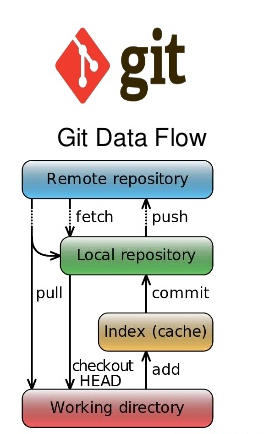
\includegraphics[scale=0.6]{git_workflow}
\caption{A summary of Git workflow taken from \href{http://www.slideshare.net/VinothKumarKannan/svn-vs-mercurial-vs-github}{here} }
\label{fig:git_workflow}
\end{figure}
Figure \ref{fig:git_workflow} encompasses a good chunk of what you need to know about Git. The following sections will show you two important examples:
\begin{itemize}
\item [1.] How to create a local repository on your computer, a remote repository on Github and synchronize the two. In particular, the \textit{init}, \textit{add}, \textit{commit} and \textit{push} commands will be exemplified. 
\item [2.] How to contribute to code in a collaborative environment.
\end{itemize}
\subsection{How to set up a local/remote repository}

\subsubsection{Create the local repository}
We begin by opening a terminal window into the folder where we want to create our repository. In this example, the repository will be in a folder named \textit{NewStudentHandout} located in the \textit{Documents} folder of a Unix system. On a Mac, the terminal command \textit{pwd} would return 
\textit{/Users/my\_username/Documents/NewStudentHandout} when executed from \textit{NewStudentHandout}. Once we have made sure that the window terminal is in the right folder, let's type
\begin{lstlisting}[language=bash, caption=Creation of the local repository]
git init
\end{lstlisting}
If everything goes well, the following should appear on the terminal window:
\begin{lstlisting}[language=bash, caption=Successful git init message ]
Initialized empty Git repository in /Users/bbercovici/Documents/NewStudentHandout/.git/
\end{lstlisting}
This command initiates the local git repository by creating the hidden directory \textit{./git} and populates it with a number of configuration files. These files are the backbone of your local repository, so make sure not to alter them.\\
As noted by Git, our local repository is empty. Note that the working directory content is unrelated to the local repository content as those are two separate entities as shown on Figure \ref{fig:git_workflow}. We thus have to use \textit{add} to add files to the index cache, and \textit{commit} this index to have those files added to our local repository.\\
Let us start with the \textit{add} command. It can be used in two different ways, as shown below (assuming that \textit{myfile.txt} does exist in the working directory):
\begin{lstlisting}[language=bash, caption=Add files to the cache ]
git add myfile.txt
# the index cache only contains myfile.txt
git add *
# the index cache now contains all files in the working directory that were not excluded in .gitignore 
\end{lstlisting}
Another useful command is \textit{status}, which highlights files depending on whether they have been modified since the last commit. Since \textit{git status} lists myfile.txt in green, we are now ready to commit it to the local repository using the following command:
\begin{lstlisting}[language=bash, caption=commit files to the local repository ]
git commit -m "first commit: myfile.txt added to the local repo"
\end{lstlisting}
The "-m" options allows us to append a message to the commit. After the content of the local repository is pushed to remote repository, the other developers will be able to read the message and quickly understand what this commit was about.

\subsubsection{Create an account on Github}
The title of this section is quite self-explanatory. Make sure you remember your username/password as you will need them shortly!
\subsubsection{Create the remote repository on Github}
Log on to Github and click on "New repository" in the drop-down list next to your profile picture as show on Figure \ref{fig:new_repo}.
\begin{figure}[H]
\centering
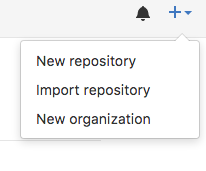
\includegraphics[scale=0.5]{new_repo}
\caption{New repository}
\label{fig:new_repo}
\end{figure}

The following window (shown on Figure \ref{fig:new_repo_settings}) allows you to choose several important settings for your remote repository.
\begin{figure}[H]
\centering
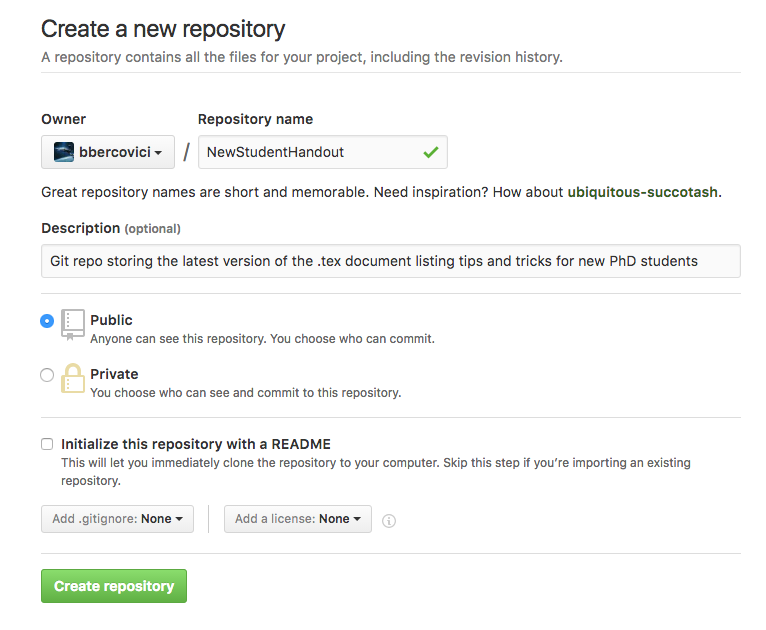
\includegraphics[scale=0.6]{new_repo_settings}
\caption{New repository settings}
\label{fig:new_repo_settings}
\end{figure}

\begin{itemize}
\item Choose whether the repository will be made public or private (the latter being only available if you have upgraded to a premium account).
\item Initialize the repository with a README.md file. \\\textcolor{red}{Leave this box unchecked if your local repository is already created, as this file can be added later on manually without risking conflicts}
\item Add a .gitignore file. This file lists all the file extensions that must be ignored by Git. Especially handy if there are specific file extensions that you never want to see included in a commit.
\item Add a license file.
\end{itemize}
When you are ready, simply click on Create Repository and proceed to the next step.
\subsubsection{Connect the local repository to the remote repository}
You should now be seeing the same page as on Figure \ref{fig:setup_options}. 

\begin{figure}[H]
\centering
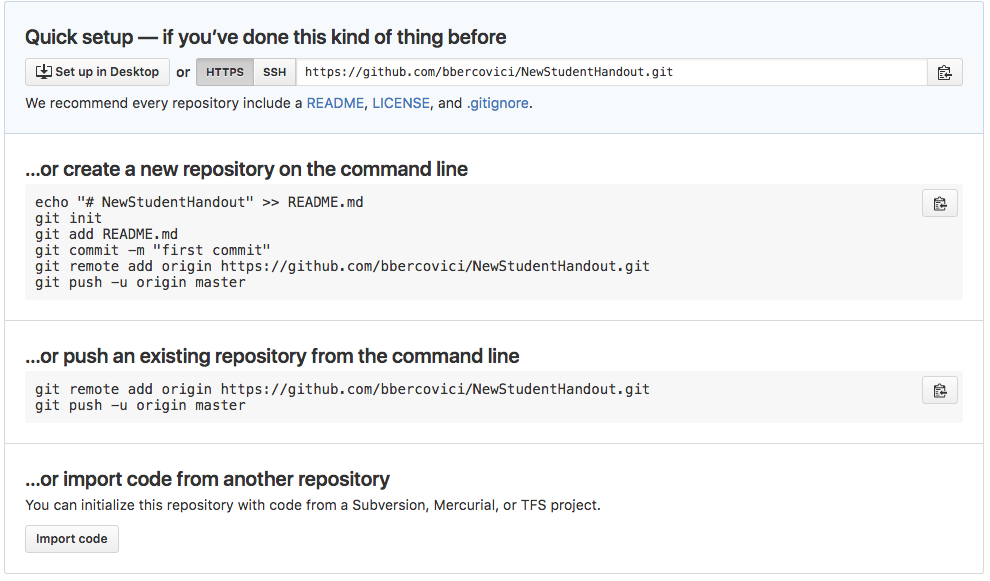
\includegraphics[scale=0.4]{setup_options}
\caption{Final setup options}
\label{fig:setup_options}
\end{figure}
The third option is what we want to do, since we have already created a remote repository. We can copy and paste the two lines under "...push an existing repository from the command line" into our terminal. Start with the following:
\begin{lstlisting}[language=bash, caption=Add the remote repository location ]
git remote add origin https://github.com/bbercovici/NewStudentHandout.git
\end{lstlisting}
This will add the remote repository address to one of the hidden configuration files. Finally, push the local repository to the remote.

\begin{lstlisting}[language=bash, caption=Push the local repository to the remote ]
git push -u origin master
\end{lstlisting}

We are now all set! We can keep working in our local directory, add files containing new content to the index using \textit{git add}, commit the changes to the local repository using \textit{git commit}, and finally pushing the changes to the remote using \textit{git push origin master} (note that the -u option was not used here). Now is also the time to create a .gitignore file and a README.md file.
\subsection{Contribute to code in a collaborative environment}
\section{\LaTeX\ }


This section walks you through the most critical, time-consuming, less-rewarding steps of  the download \& installation of the LaTeX distribution, to the point where you can compile and edit your own documents. 
\paragraph{}
There are two things that you need in order to do so:
\begin{itemize}
\item[1.] The \LaTeX\ distribution: the (huge) software package that will compile your raw .tex document and turn them into  neat pdf documents.
\item[2.]  The TeX editor. This is the software that you will use to create and edit .tex documents. It also provides an interface with the compiler.
\end{itemize}
\paragraph{}
The procedure is slightly different depending on whether you are using Windows or MacOS.

\subsection*{Retrieving the \LaTeX\ Distribution }

\subsubsection*{Windows}
Two versions of the \LaTeX\ distribution installer are available on the  \href{http://www.miktex.org/download
}{\textcolor{blue}{MikTeX website}}



\begin{itemize}
\item If your computer is less than two years old,
you can download the MiKTeX 2.9.5870 Net Installer 64-bits executable
\item If you are not sure whether you can run the 64-bits executable, 
download the MiKTeX 2.9.5870 Net 32-bits executable 
\end{itemize}


\begin{itemize}
\item[1.] Run the installer once the file is downloaded.
\item[2.] When asked, click ‘Download MiKTeX’ to download the distribution.
\item[3.] When asked whether the executable should download the Basic or Complete MiKTeX distribution, choose Complete
\item[4.] Choose the folder where the installation files will be downloaded
\item[5.] Pick a download source geographically close from CU in the server list that should pop up
\item[6.] Start the download...
\end{itemize}
...which might take a while...
\begin{itemize}
\item[7.] Once the download is over, go to the folder where you saved the \LaTeX\ distribution files. Look for setup-2.9.3959.exe (the only executable file in this folder) and run it.
\item[8.] Once the installation process is over, you have a complete \LaTeX\ distribution installed on your PC and are almost good to go!
\end{itemize}

\subsubsection*{MacOS}
\href{https://tug.org/mactex/mactex-download.html}{\textcolor{blue}{The MacTex distribution}} can be found there. Click on the link at the center of the page to get the whole distribution. The file weighs 2.5 GB so the download might take a while .

\subsection*{Getting the Tex Editor}
From my own experience, I strongly recommend
\href{http://www.xm1math.net/texmaker/}{\textcolor{blue}{Texmaker}}. The interface is neat and the autocomplete functionality (that predicts the rest of the command you are typing) rocks.\\
This software works on Windows, MacOS and Linux. The version you need can be found on the download page. Installing Texmaker does not require any special instructions so you should be fine!

\subsection*{Editing and compiling this tutorial}

First of all, download the following \href{https://drive.google.com/file/d/0Bzf79yzZcPJJNVhKNFBxWGs1aEE/view?usp=sharing}{archive} and extract it into a folder of your choice.

The \textit{preamble.tex} file lists all the packages that are needed in order to compile some commands that would otherwise be unknown to the Latex compiler. I have been using Latex and constantly updating this list of packages for nearly 4 years, so it should be comprehensive enough now\footnote{The \textit{float} package that you will see listed in the preamble is one of these packages that come in handy. Without it, including figures in your document can lead to layout disasters... }.

Once this is done, open Texmaker. Figure \ref{fig:texmaker_menu} shows what you should see as you have no tex document currently opened.

\begin{figure}[H]
\centering
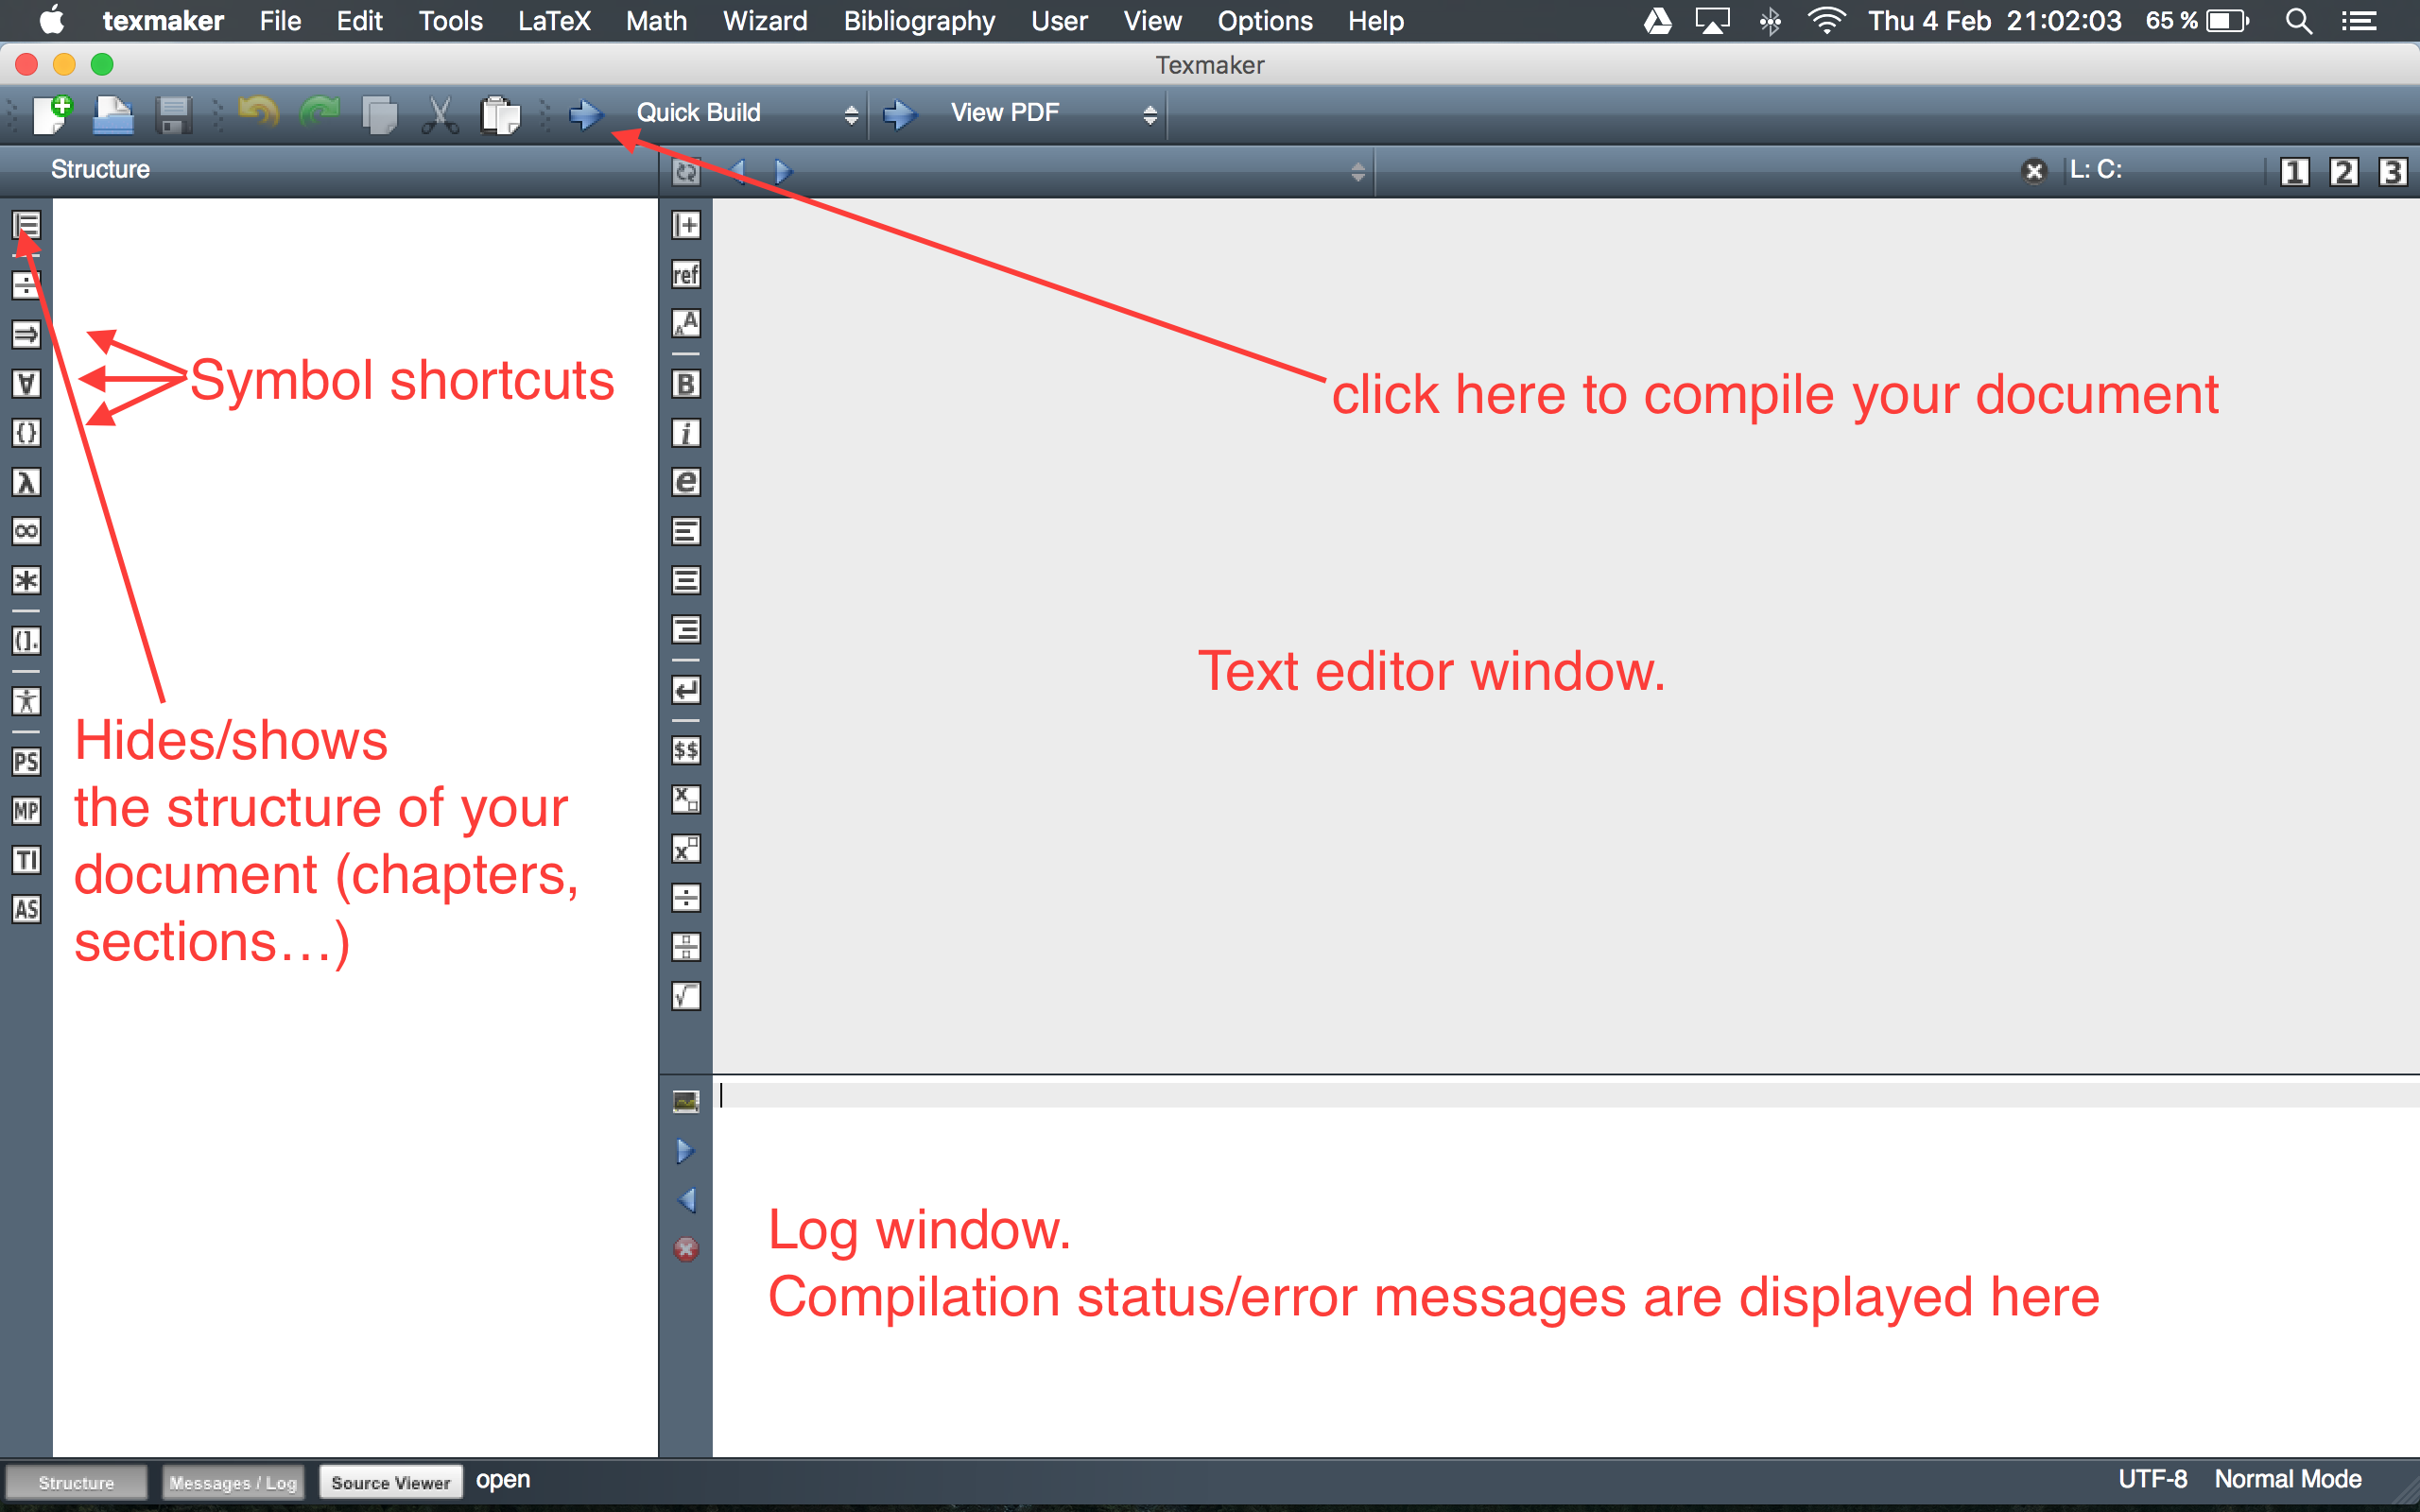
\includegraphics[scale=0.38]{texmaker_menu}
\caption{Main menu}
\label{fig:texmaker_menu}
\end{figure}

Opening the tutorial.tex file should get you the same view as on Figure \ref{fig:opened_document}:

\begin{figure}[H]
\centering
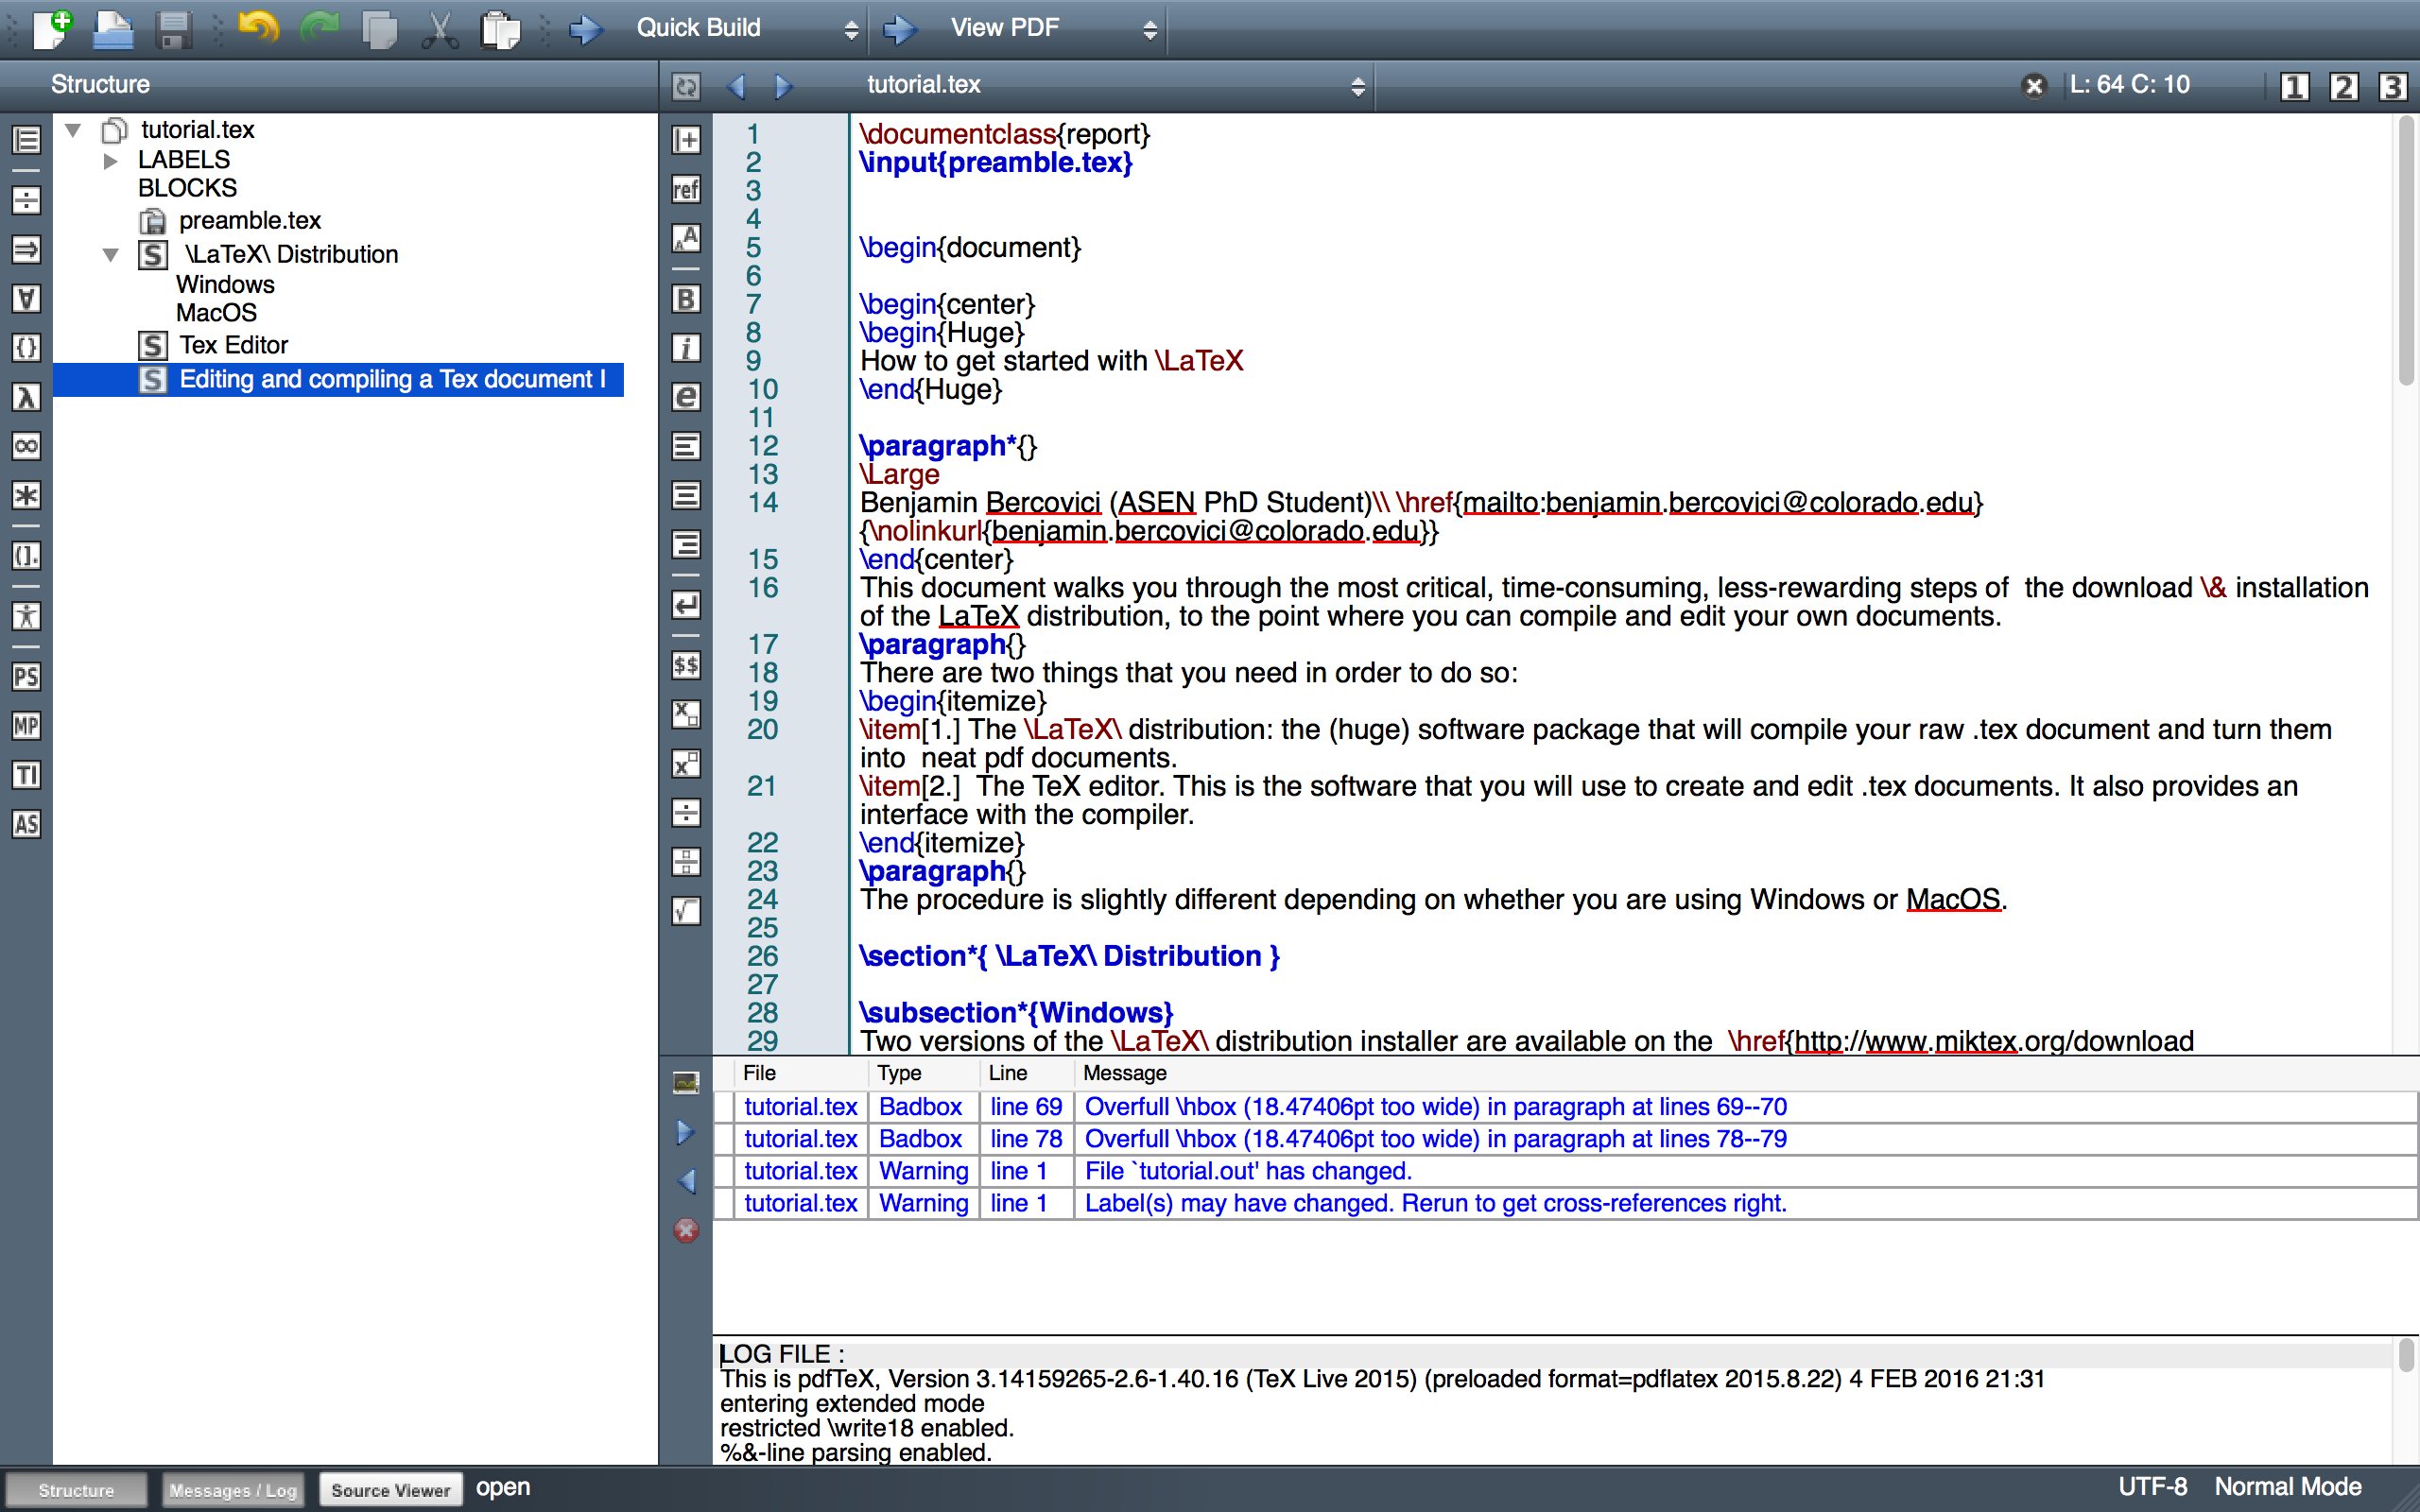
\includegraphics[scale=0.38]{opened_document}
\caption{Texmaker displaying the \textit{tutorial.tex} file. Note that the document structure automatically appears on the left side of the window}
\label{fig:opened_document}
\end{figure}
If you take a look at the very top of the document, you will recognize the \textit{preamble.tex} file that I mentioned before. The \textit{$\setminus$input\{preamble.tex\}} command will - as the name suggests - have \textit{tutorial.tex} including the content of \textit{preamble.tex}. It is equivalent to copying the content of \textit{preamble.tex} and pasting it into \textit{tutorial.tex}. Because the latter would be rather messy, listing all the packages you will use in an external file and using the input command is a much better practice.\\

Note that everything that begins with a $\setminus$\footnote{The key that corresponds to this symbol is the one right above the Enter/Return Key.} is a \LaTeX\ command. This $\setminus$ tells the compiler that whatever follows this symbol has to be interpreted. Plain text is just considered as is. \\
Clicking on the \textit{Quick Build} button will run the compiler, that will process the .tex file and generate a \textit{tutorial.pdf} document in the same folder as the \textit{tutorial.tex} file

\subsection*{Maths and \LaTeX }
There are thousands of tutorials available on the web addressing this topic. The greatest understatement of the day would be to say that \LaTeX\ is really well suited to maths typesetting. Several examples based off former homeworks of mine are available \href{https://drive.google.com/file/d/0Bzf79yzZcPJJSnJKOFdrLVhtSG8/view?usp=sharing}{there}.

I strongly encourage you to open the document, compile it, see the pdf output, and then take a closer look at the .tex file to understand how mathematical expressions are formatted.
\subsection*{Resources}
Dr. Schaub has listed a number of references on \href{http://hanspeterschaub.info/AVS-LaTeX.html}{his website} which I encourage you to use. There is in particular a Latex cheat sheet that could come in handy.  

\section{Asymptote}
\subsection{Brief description}
\href{http://asymptote.sourceforge.net/}{Asymptote} is "a powerful descriptive vector graphics language that provides a natural coordinate-based framework for technical drawing." In other words, it is a compiled language that generates .eps or .pdf representing any 2D or 3D scene parametrized mathematically. Its hybrid syntax borrows from Python, C and Latex, which can be a bit bewildering at first. Raw asymptote code is customarily stored in the form of a .asy file, which can be edited using the text editor of your choice.
The installation procedure depends on the platform you are using:
\begin{itemize}
\item MacOS X: Asymptote is already shipped with MacTex, so there is nothing to do besides retrieving the Latex distribution
\item Windows: Download the latest executable file from \href{https://sourceforge.net/projects/asymptote/files/}{the official Asymptote page}. Make sure to have a running Latex distribution before attempting to run Asymptote!
\item Linux: Similarly to MacOS X, Asymptote is shipped with the TexLive distribution.
\end{itemize} 
Asymptote files can be compiled directly from a Unix terminal. Simply type \textit{asy myfile.asy} to compile the file and generate the output which by default will be named \textit{myfile.pdf} or \textit{myfile.eps}. The output format can be set using the \textit{settings.outformat="pdf";} instruction in the asy file. On Windows, compilation can be taken care of by TexMaker.
\subsection{Examples}
Two Asymptote output files are presented below, to demonstrate the 2D and 3D capabilities of the language. Figure \ref{fig:flyby} represents a planetary flyby where the input angles are prescribed to their real value. The trajectory that is displayed is a conic (an hyperbola in this case) which corresponds to the true Keplerian orbit expected in this case.
\begin{figure}[H]
\centering
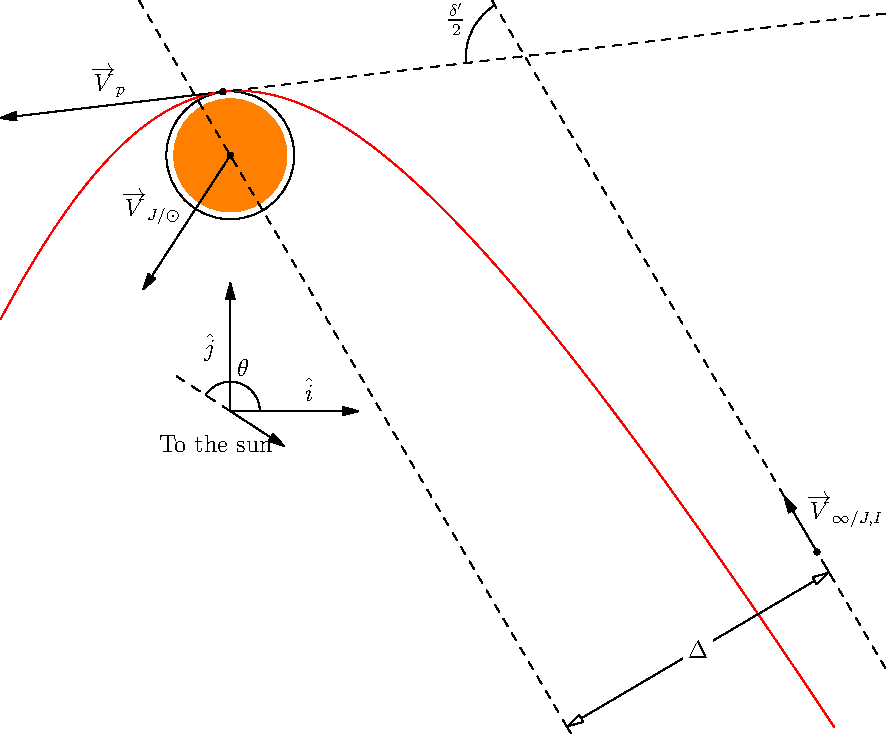
\includegraphics[scale=0.6]{flyby.pdf}
\caption{Planetary flyby (2D scene)}
\label{fig:flyby}
\end{figure}
The example shown on Figure \ref{fig:ECI_to_body} is another illustration of Asymptote capabilities. Here, the body frame of a spacecraft is represented relative to an inertial frame. The spacecraft attitude is parametrized in terms of a set of 321 Euler angles (yaw, pitch, roll) that the user can edit. Recompiling the .asy file for a new attitude will generate the same scene with a different orientation, without requiring the user to edit manually the location of every single satellite feature.
\begin{figure}
\centering
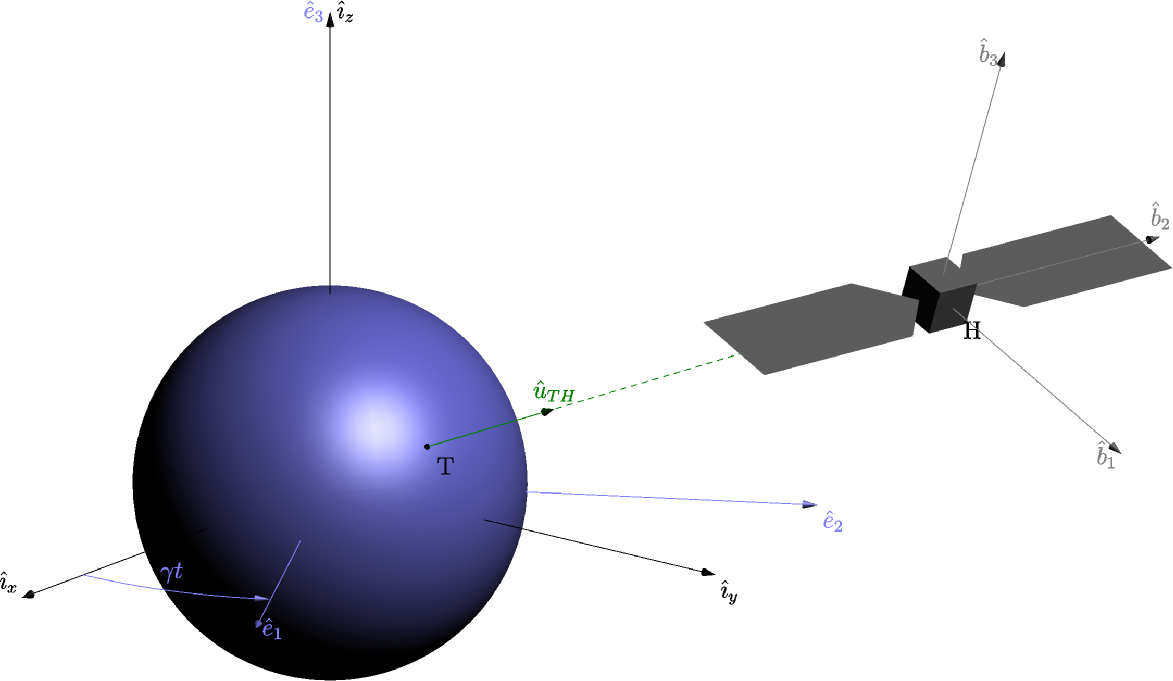
\includegraphics[scale=0.5]{ECI_to_body.pdf}
\caption{Satellite body-frame to inertial frame (3D scene)}
\label{fig:ECI_to_body}
\end{figure}
\subsection{More examples}
The best compilation of examples I have found to date is probably \href{https://drive.google.com/file/d/0Bzf79yzZcPJJc0dWTHNZMkhqTGc/view?usp=sharing}{this one for 2D examples} and
\href{https://drive.google.com/file/d/0Bzf79yzZcPJJYld2cnhqWXZNU28/view?usp=sharing}{ this one for 3D examples}. As the reader will soon notice, these resources are unfortunately not in English. This being said, they are quite self explanatory due to the ubiquitous use of English in the Asymptote language in addition to the (almost) comprehensive list of Asymptote routines they provide. English documentation files, quite comprehensive but maybe less exhaustive can also be found \href{http://asymptote.sourceforge.net/asymptote.pdf}{here} and another one \href{https://math.uchicago.edu/~cstaats/Charles_Staats_III/Notes_and_papers_files/asymptote_tutorial.pdf}{here}.






\end{document}
